\documentclass[a4paper]{article}

\usepackage{amssymb}
\usepackage{euscript}
\usepackage{graphicx}
\graphicspath{{pics/}}
\usepackage{color}
\usepackage{epsfig}
\usepackage{fullpage}
\usepackage[colorlinks=true]{hyperref}
\usepackage{eurosym}

\oddsidemargin -1cm
\topmargin -1cm
\textwidth 18cm
\textheight 26cm
\pagestyle{empty}

\newcommand{\image}[3]{
\begin{figure}[#1]
\begin{center}
\includegraphics{full_#2.eps}
\caption{\small#3}
\label{image:#2}
\end{center}
\end{figure}
}


\twocolumn
\begin{document}

\section*{Thermometers for dilution fridges (V.Zavjalov, 11.2018)}

The goal is to make standard thermometers for use in dilution fridges. I
use carbon OHMITE resistors (OD/OF series)~\cite{ohmite_catalog}, which
are claimed to be good thermometers at millikelvin
temperatures~\cite{therm_paper}. The series OD and OF have different
sizes (diameter $2.5$~mm and~$3.8$~mm and length~$7$~mm and~$10$~mm
respectively). I grind resistors down to approximately $0.7$~mm thickness
and glue it in a slit in a copper box using Stycast 2850. This provides
a good thermal contact with the box, mechanical stability, and protection
against moisture.

\begin{center}
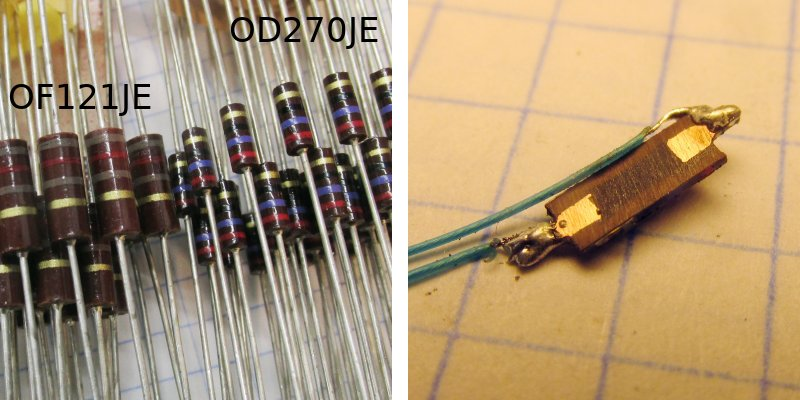
\includegraphics[width=\linewidth]{img/res.jpg}
\end{center}

Copper boxes are ordered in Schaeffer-AG company~\cite{schaeffer}.  The
box has $30\times30\times5$~mm size. It contains a~$20\times18\times3$~mm
compartment for RC lowpass filters, a $1\times16\times4$~mm slit for the
resistor and a~$16\times7\times3$~mm additional compartment which can be
used for sample chips. Holes are compatable with standard~$20\times20$ M4
hole grid on BlueFors refrigerator plates. Drawings in FPD format are
available~\cite{box_drawings}, price was 315\euro{} for 10 boxes and 10
lids.

\begin{center}
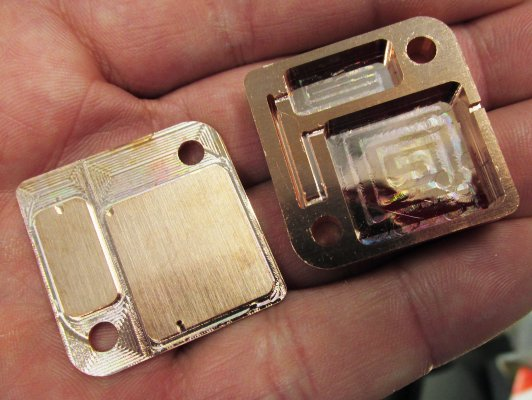
\includegraphics[width=\linewidth]{img/box.jpg}
\end{center}

PCBs for filters are ordered in Multi-CB company~\cite{multi-cb}. Price
is 75\euro{} for 10 boards with two different filters and two small
sample plates each. Kicad project~\cite{filterpcb-kicad} and Gerber
files~\cite{filterpcb-gerber} are available.

To connect thermometers to BlueFors 4-pin sockets we use inserts
of LEMO {\tt FFA.0S.304.CLAC44} connectors (Farnell number: 2442870).

\begin{center}
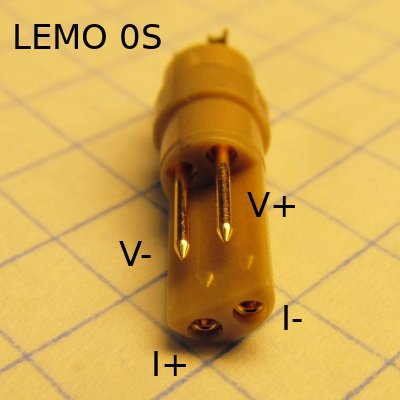
\includegraphics[width=3.5cm]{img/conn.jpg}
\end{center}

\subsection*{List of devices}

\noindent
\begin{tabular}{|ll lll l|}\hline
N& Resistor& $R_0$ & $R_1$ & $R_2$ & \\
\hline
2018-11-02 N1&OD270JE& 27  & 56  & 56.0&\\
2018-11-02 N2&OD270JE& 27  & 59  & 64.4&\\
2018-11-02 N3&OF121JE& 120 & 231 & 277&\\
\hline
\end{tabular}
\medskip

Here $R_0$, $R_1$, and $R_2$ are nominal resistance, resistance after
grinding, and resistance after soldering and glueing. Change during
glueing probably means that contacts with carbon in the resistor
after grinding are not stable.

\begin{thebibliography}{}

\bibitem{ohmite_catalog}
Ohmite OD/OF series datasheet,\\
\url{https://www.ohmite.com/assets/docs/res_od_of_oa.pdf}

\bibitem{therm_paper}
N. Samkharadze, A. Kumar, G. A. Cs{\'a}thy,
A New Type of Carbon Resistance Thermometer with.Excellent Thermal Contact at Millikelvin Temperatures,
{\it JLTP}, {\bf 160}, 246--253 (2010),\\
\url{https://doi.org/10.1007/s10909-010-0192-5}

\bibitem{schaeffer}
Schaeffer-AG company,\\
\url{https://www.schaeffer-ag.de/en/}

\bibitem{box_drawings}
Box drawing in FrontPanel Disigner format,\\
\url{https://github.com/slazav/he3notes/raw/master/20181105-mk_therm/suppl/box_v1.zip}

\bibitem{multi-cb}
Multi-CB company,\\
\url{https://portal.multi-circuit-boards.eu}

\bibitem{filterpcb-kicad}
Filter PCB, KiCAD project,\\
\url{https://github.com/slazav/he3notes/tree/master/20181105-mk_therm/suppl}

\bibitem{filterpcb-gerber}
Filter PCB, Gerber files for ordering,\\
\url{https://github.com/slazav/he3notes/raw/master/20181105-mk_therm/suppl/filter\_pcb_v1.zip}

\end{thebibliography}
\end{document}
